\setAuthor{Marko Tsengov}
\setRound{piirkonnavoor}
\setYear{2023}
\setNumber{G 8}
\setDifficulty{8}
\setTopic{TODO}

\prob{Süvend ja kera}
\begin{wrapfigure}{r}{0.35\textwidth}
\vspace{-1em}
  \begin{center}
    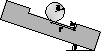
\includegraphics[width=1\linewidth]{2023-v2g-08-yl.pdf}
  \end{center}
  \vspace{-2em}
\end{wrapfigure}

Tasandil on silindrikujuline süvend raadiusega $r$ ning sügavusega $h$, mis on risti tasandi pinnaga. Süvendi sisse asetatakse kera raadiusega $R$, nii et kera puudutab süvendi keskpunkti ja kera on algselt paigal. Tasand on maapinna suhtes kaldus nurga $\theta$ võrra. Millist tingimust peavad rahuldama antud suurused, et kera saaks mingi arvu põrgete järel süvendist välja hüpata? Võib eeldada, et hõõrdumist ei toimu, põrked on täielikult elastsed, pindade ebatasasuste tõttu on põrkesuunad vähesel määral juhuslikud ning $h < R$.


\hint

\solu
Juhul $\theta > \SI{90}{\degree}$ kukub kera kindlasti tasandilt maha.

Olgu $C \equiv \sqrt{(R - h)^2 + r^2}$. Kui $R = C$, siis puudutab kera korraga nii süvendi põhja kui ka äärt. Seega juhul $R > C$ puudutaks kera ainult süvendi äärt (mis pole ülesandes antuga kooskõlas).

Kui $R \leq C$, libiseb kera esmalt mööda süvendi põhja kauguse $C - R$ võrra, kogudes kineetilist energiat potentsiaalse energia arvelt. Seejärel kera põrkab servalt -- võib-olla korduvalt -- kuni ta kas ületab süvendi serva või jääb (aeglaselt sumbuvate põrkamistega) süvendisse. Selleks, et kera süvendist väljuks, peaks algne potentsiaalne energia olema suurem potentsiaalsest energiast, mille kera saavutab, kui see puudutab serva ning selle masskese on täpselt puutepunkti kohal. Teisisõnu peab kera sellises olekus olema madalamal kui algolekus. Kõrguste vahe saame leida, liigutades kera masskeskme mõtteliselt:
\begin{enumerate}
    \item Kera algsesse puutepunkti: $\Delta H = -R\cos\theta$
    \item Süvendi serva alumisse punkti: $\Delta H = -r\sin\theta$
    \item Süvendi serva ülemisse punkti (süvendi ääre peale): $\Delta H = h\cos\theta$
    \item Süvendi ääre kohale, nii et kera masskese on täpselt puutepunkti kohal: $\Delta H = R$
\end{enumerate}
Liites kõrguste vahed kokku, saame
\begin{equation*}
    \Delta H = -R\cos\theta - r\sin\theta + h\cos\theta + R = R-r\sin\theta-(R-h)\cos\theta
\end{equation*}

Kera saab süvendist väljuda, kui $\Delta H \leq 0$, st
\begin{equation*}
    R-r\sin\theta-(R-h)\cos\theta \leq 0
\end{equation*}

Ei ole oluline, kas õpilane kasutab tingimuses ranget ($<$) või mitteranget ($\leq$) võrratust.
\probend